\documentclass{standalone}
\usepackage{circuitikz}
\usepackage{schemabloc}

\begin{document}
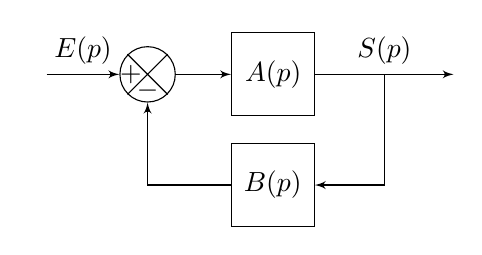
\begin{tikzpicture}
\sbEntree{E}
\sbComp{comp}{E}
\sbRelier[$E(p)$]{E}{comp}
\sbBloc{B1}{$A(p)$}{comp}
\sbRelier{comp}{B1}
\sbSortie[5]{S}{B1}
\sbRelier[$S(p)$]{B1}{S}
\sbDecaleNoeudy[4]{comp}{G}
\sbBloc[3]{B2}{$B(p)$}{G}
\sbRelieryx{B1-S}{B2}
\sbRelierxy{B2}{comp}
\end{tikzpicture}
\end{document}